\subsection{Задача 1}

Субдифференциальный метод Ньютона вернул следующий результат:
\begin{equation}
\mathbf{x} = 
\begin{pmatrix}
1.000 \\
[1.444, 0.636] \\
[0.667, 1.273]
\end{pmatrix}
\end{equation}

Решение производилось с точностью до третьего знака. Невязка решения равна нулю (найденное решение является точным).

\begin{remark}
	Подразумевается ненулевая невязка при подстановке решения вплоть до последнего полученного знака. Однако предъявляется решение именно вплоть до третьего знака, поскольку запрос в методе был именно таковым. Однако, как мы знаем из теоретического раздела, данный метод отыскивает точное решение полиэдральных функций, поэтому полученный результат является отнюдь не удивительным, а закономерным.
\end{remark}

\subsection{Задача 2}

В качестве начального вектора был взят вектор, приложенный в письме (см. \ref{app}).

Сопутствующие задачи с квадратными матрицами были решены с помощью метода, использующего знаково-блочные матрицы. В результате был получен следующий вектор:
\begin{equation}
\mathbf{x}=
\begin{pmatrix}
[0.558, 0.442] \\
[0.697, 0.802] \\
[1.104, 0.895] \\
[0.960, 1.039] \\
[0.751, 0.748] \\
[0.282, 0.717] \\
[0.374, 0.125] \\
[0.523, 0.476] \\
[0.692, 0.807] \\
[0.695, 0.804] \\
[0.469, 0.530] \\
[0.267, 0.232] \\
[0.077, -0.077] \\
[0.321, 0.178] \\
[0.752, 0.247] \\
[0.539, 0.460] \\
[0.408, 0.091] \\
[0.155, -0.155] \\
[2.194, -2.194] \\
[0.389, 0.110] \\
[0.880, 0.119] \\
[0.493, 0.506] \\
[0.673, -0.173] \\
[0.269, -0.269] \\
[0.282, 0.217] \\
[0.629, 0.370] \\
[0.816, 0.683] \\
[0.745, 0.754] \\
[0.390, 0.609] \\
[0.078, 0.421] \\
[0.527, 0.472] \\
[1.382, 0.117] \\
[1.149, 0.850] \\
[1.113, 0.886] \\
[0.795, 0.704] \\
[0.280, 0.719]
\end{pmatrix}
\end{equation}

Правый столбец сгенерирован следующим образом: матрица из файла \texttt{matrix\_n\_phi\_1.txt}, помноженная на вектор $x^{(0)}$ (см. \hyperref[app]{``Приложения''}), определяет $\mathrm{mid} \mathbf{b}$. Вектор объинтерваливается по формуле:

\begin{equation}
\mathbf{b}_i = [\mathrm{mid} \mathbf{b}_i - 0.05 \cdot (i \; \mathrm{mod} \; 7 + 1),
\mathrm{mid} \mathbf{b}_i + 0.05 \cdot (i \; \mathrm{mod} \; 7 + 1)]
\end{equation}

Найденное решение удовлетворяет 144 уравнениям из 256.

Начальный вектор $x^{(0)}$ пересекается с итоговым результатом по 17 компонентам из 36.

Произведение матрицы на вектор-решение не может поместиться на одну страницу данного отчёта, поэтому оно представлено в отдельном файле. Ссылку можно найти в \hyperref[app]{приложениях}.

На следующем графике демонстрируется, как соотносятся компоненты найденного решения и оригинального вектора. Абсцисса соответствует номеру компоненты, ордината -- значению.

\begin{figure}[H]
	\begin{center}
		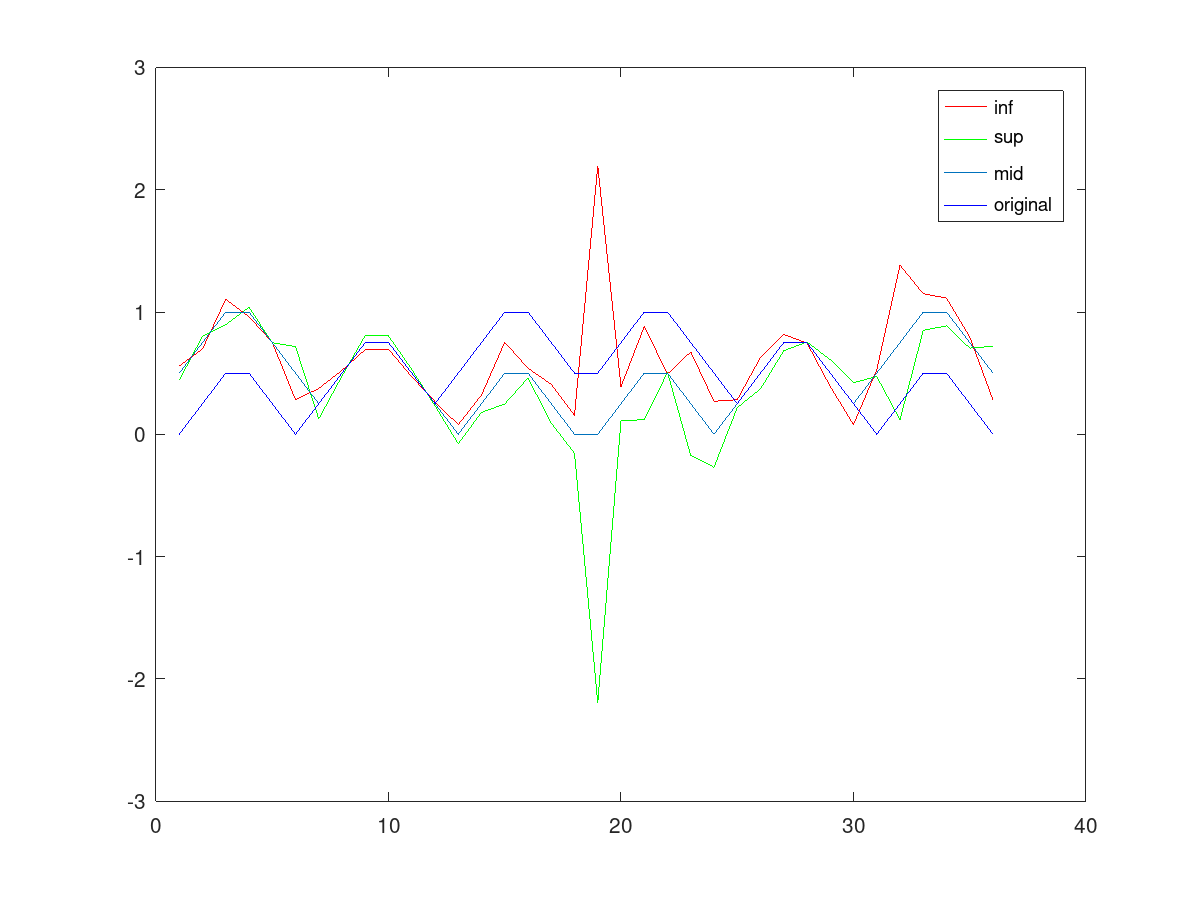
\includegraphics[scale=0.4]{subdiff}
		\caption{$\mathbf{x}, x^{(0)}$}
	\end{center}
\end{figure}